% Chapter3

\chapter{Konzept} \label{chapter:architecture}
Die Abfolge der Arbeitsschritte für die modellbasierte Entwicklung der Steuerung einer Chargenprozessanlage sieht wie folgt aus.
\begin{figure}[h!]
		\centering
		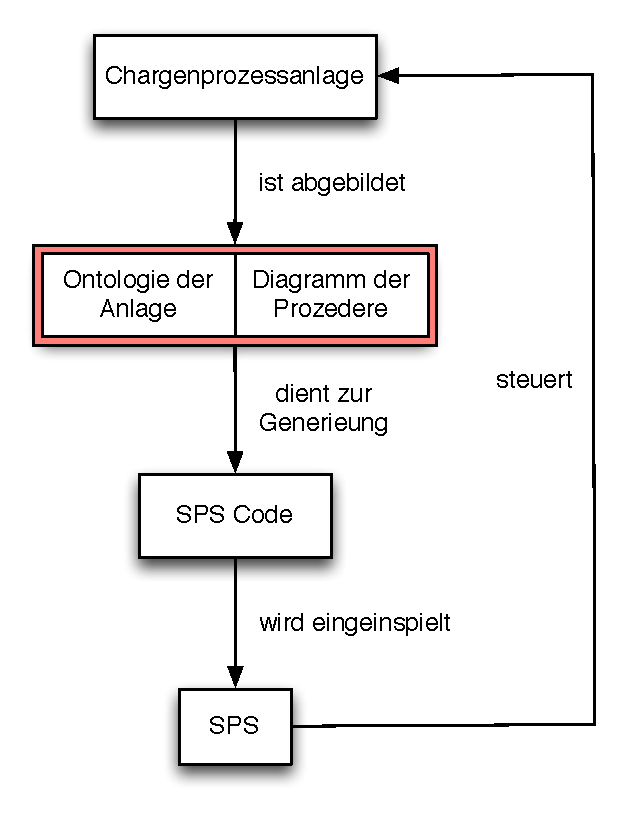
\includegraphics[width=0.37\textwidth]{graphics/konzept/konzept_new.pdf}
		\caption{Konzept für die modellbasierte Entwicklung der Steuerung}
		\label{fig:konz_konzept_new}
\end{figure} \\
%\todo{modellbasierte entwicklung bei austausch/erweiterung}
Es beginnt mit einer Produktionsanlage, wobei es sich um eine Chargenprozessanlage handelt, die in einer Ontologie abgebildet wird. Die Ontologie und das Diagramm der Prozeduren beinhalten die nötigen Daten, die gebraucht werden, um im weiteren Schritt den Code für die \ac{SPS} zu generieren. Dieser Code ist nach dem IEC 61512 Standard genormt. Nachdem der Code in die \ac{SPS} eingespielt wird, kann die Chargenprozessanlage gesteuert werden. 
In diesem Kapitel wird jeder Schritt, der im Kreislauf von Abbildung~\ref{fig:konz_konzept_new} enthalten ist, genauer elaboriert und in Perspektive zu dem entwickelten Konzept gebracht.
\section{Produktionsanlage}
Für eine Anlage gibt es gewisse Parameter, die beim konzeptionellen Entwurf beachtet werden müssen. Für die gestellten Anforderungen wie etwa funktionale Parallelität sowie für die zukünftig darauf aufbauenden Projekte ist es unentbehrlich, dass diverse Redundanzen vorhanden sind. Eine Voraussetzung ist jedenfalls eine Vielzahl an Hauptleitungen. Durch diese kann erst ermöglicht werden, zwei Arbeitsschritte parallel auszuführen. Das noch folgende Vorhaben, einen Wegfindungsalgorithmus zu integrieren, ist obendrein nur nutzbringend, wenn mehrere, durch die Redundanz gebotene Wege zur Auswahl stehen. Ebenso ist die Disponibilität von mehr als einer Pumpe eine essentielle Bedingung. Dadurch kann die Anlage bei der Eventualität eines Ausfalls einer Pumpe diese vollständig kompensieren. Die Ansteuerung jeder einzelnen Funktion muss somit stets von zumindest einer anderen Pumpe durchführbar sein. Zudem ist es vorgesehen, auf ausgewählten Routen die Steuerung mit Hilfe der Schwerkraft durchzuführen.\\

%Ein Ziel der Anlage muss sein, eine möglichst hohe Effizienz mit der modellbasierten Entwicklung zu erreichen.\\
\begin{figure}[h!]
		\centering
		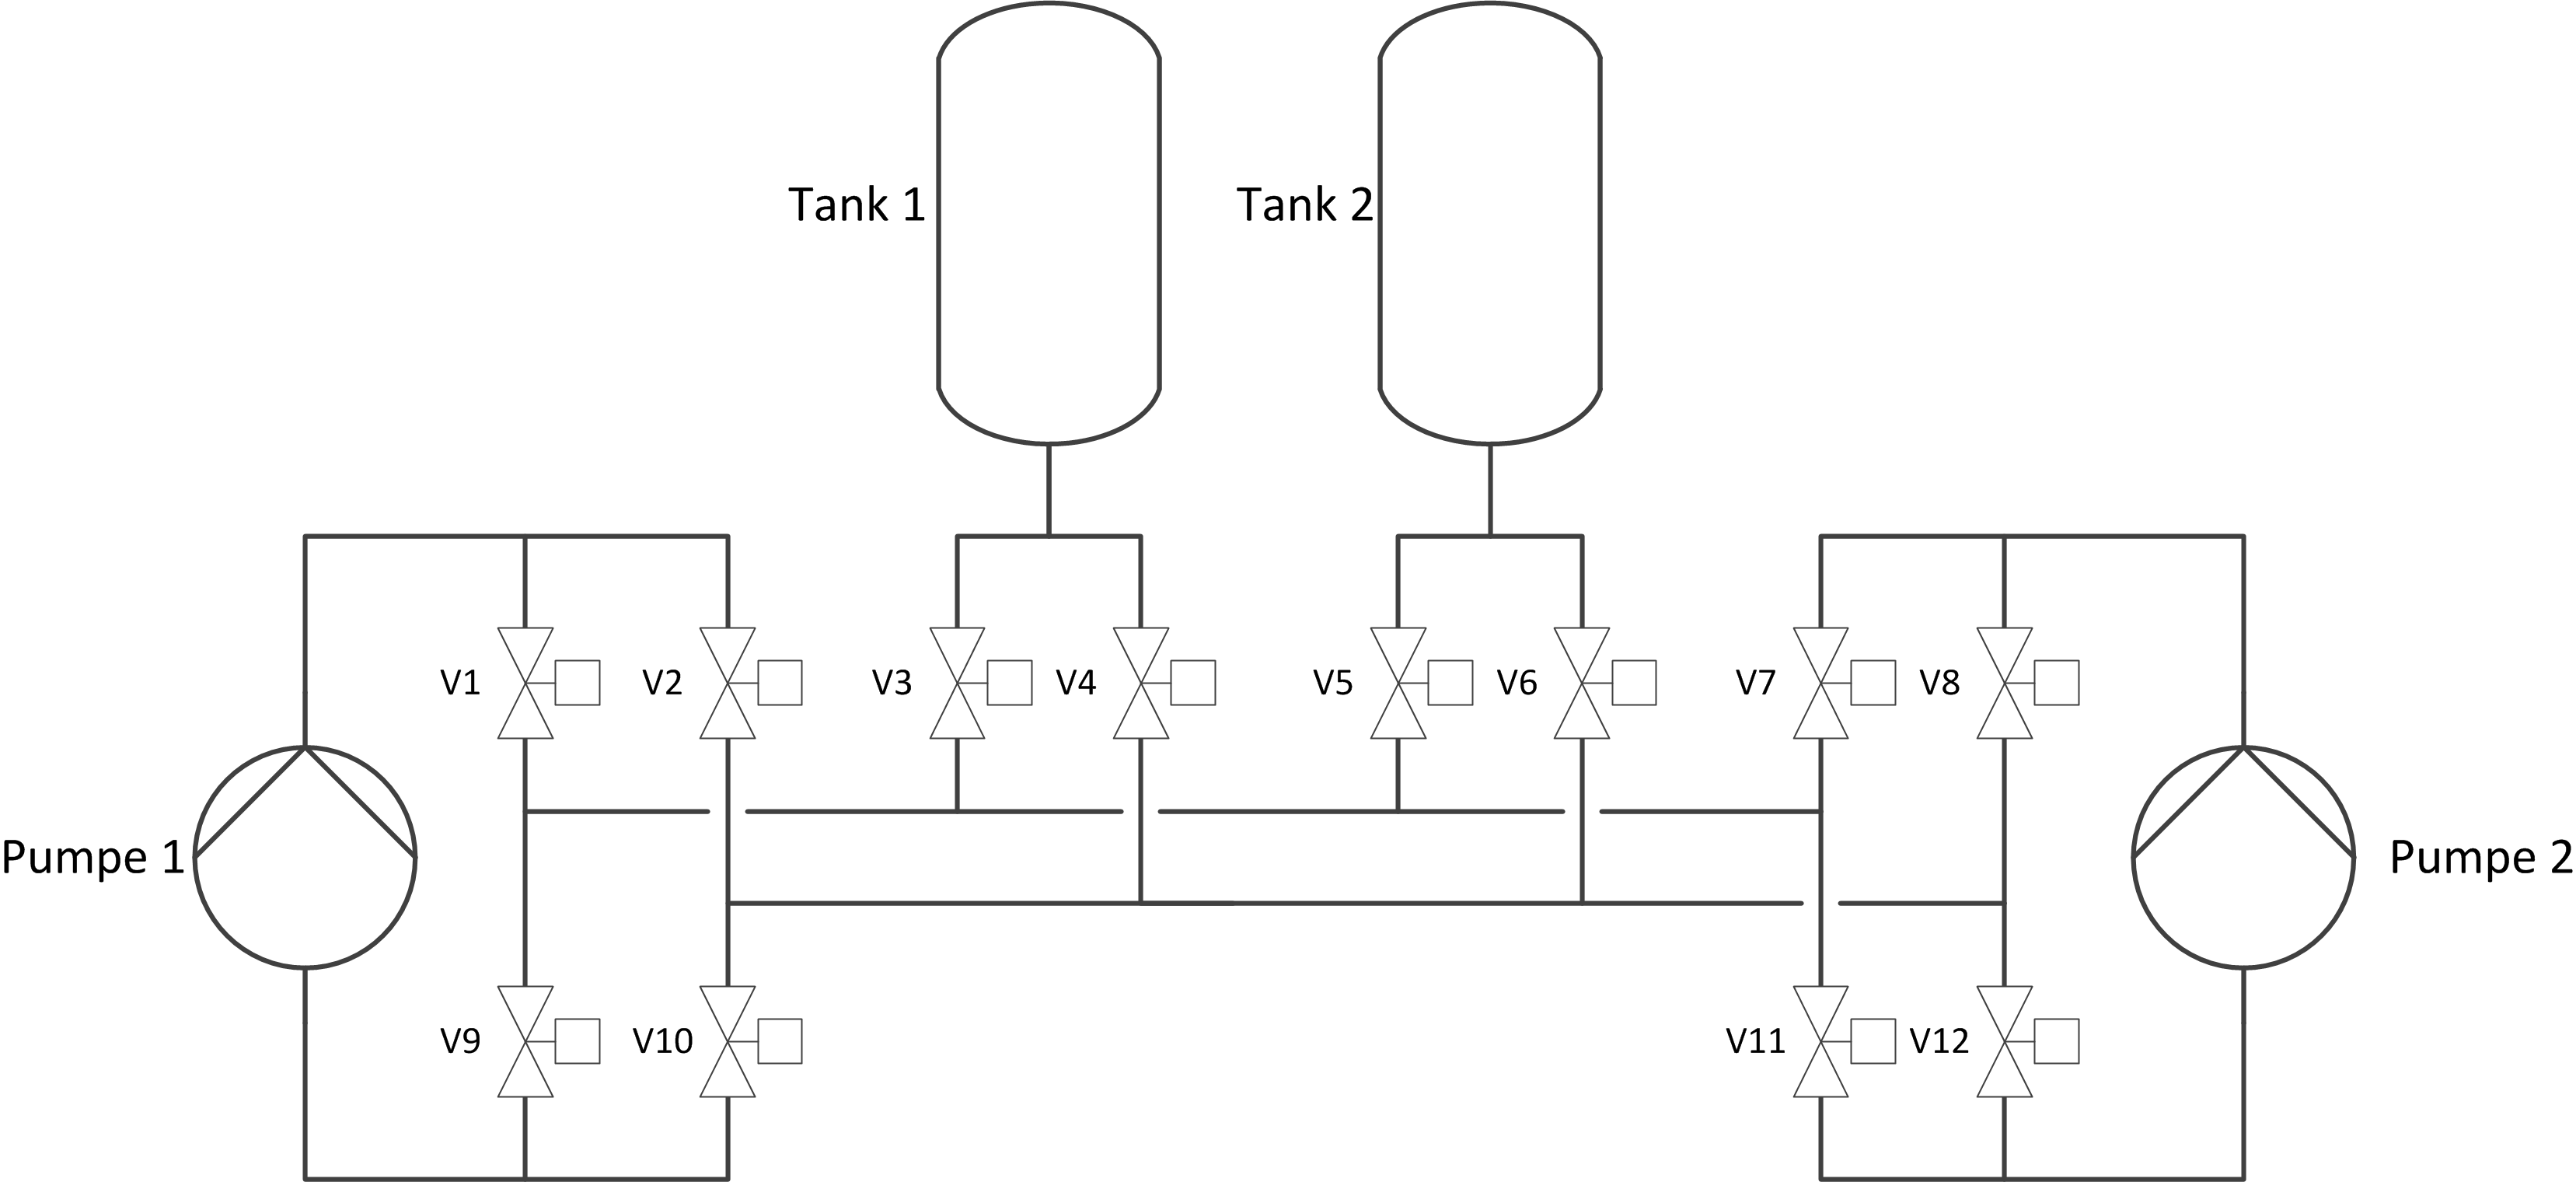
\includegraphics[width=1\textwidth]{graphics/konzept/RI_K.png}
		\caption{Konzept einer Anlage mit Redundanzen}
\end{figure}
\section{Informationskonzept}

Um eine Codegenerierung zu ermöglichen werden zwei Informationsquellen gebraucht. Einerseits einen Ontologie zur Speicherung der Informationen der Produktionsanlage und andererseits ein Aktivitätsdiagramm zur Darstellung der Prozeduren. 
Die Daten der Ontologie werden über den Namen der erstellen Identitäten (Datensätze) den Daten des Aktivitätsdiagramm zugeordnet.
Durch die Ontologie und dem Aktivitätsdiagramms werden die Informationen bereitgestellt, die für die Codegenerierung nötig sind.
\subsection{Ontologie der Chargenprozessanlage}
Hierbei handelt es sich um die Speicherung der Daten der Produktionsanlage in einer Ontologie. Je genauer diese abgebildet ist, desto mehr kann automatisch generiert werden. Wenn zum Beispiel Maximal- und Minimalwerte einfließen, können diese berücksichtigt werden.
Eine Ontologie, die eine Chargenprozessanlage abbildet, kann folgendermaßen aussehen. 
\begin{figure}[hbt!]
 \centering
  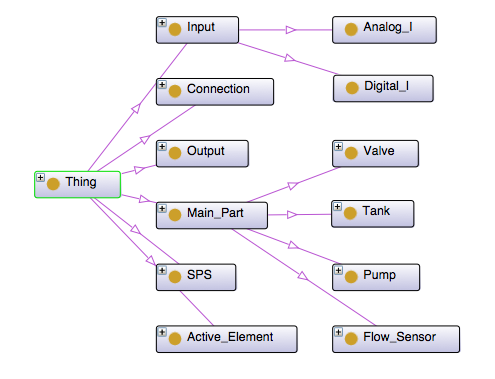
\includegraphics[width=0.6\textwidth]{graphics/stateoftheart/Ontology_Aufbau}
  \caption{Aufbau einer Ontologie}
  \label{fig:konz_Aufbau_Ontologie}
\end{figure}\\
%Die Verbindungen zwischen den Klassen (In Abbildung 3.2. die Vierecke)
In Abbildung~\ref{fig:konz_Aufbau_Ontologie} ist eine grafische Darstellung einer beispielhaften Ontologie einer Chargenprozessanlage zu sehen. Es wird zwischen „Active Element“, welches ein elektrisches Element beschreibt und „Main\_Part“ unterschieden. Unter „Main\_Part“ würden Elemente fallen die z.B. mit Rohren mit anderen Element verbunden sind.
\\\\
Damit bei der Codegenerierung ein hoher Automatisierungsgrad  erreicht werden kann, müssen möglichst viele Daten abgespeichert werden. In einer Ontologie können unteranderem Klassen (Classes), Eigenschaften von Klassen (Object Properties) und Verbindungen zwischen Klassen (Data Properties) definiert werden (siehe Kapitel 2.9.3 „Ontologie“). Dies wird sich zu Nutze gemacht um die Produktionsanlagen sehr genau abzubilden. Damit die Codegenerierung best möglich umgesetzt werden kann, werden folgende Daten einer Chargenprozessanlage gebraucht:

\begin{itemize}
  \item Elektrische Elemente (Pumpe, Ventil, \ac{SPS})
  \item Nicht- Elektrische Elemente (Tank, Reaktor)
  \item Eigenschaften der Elemente (Maximal- Minimalwert, Analog/Digital)
  \item Verbindung zwischen den Elementen (Eins-zu-Eins, Kreuzung)
\end{itemize}

\textbf{Elektrische Elemente}\\
Diese Kategorie beinhaltet alle Elemente die einen I/O Port in einer \ac{SPS} brauchen, um mit Strom versorgt und angesprochen zu werden. Darunter können zum Beispiel eine Pumpe, ein Ventil, jegliche Art von Sensor aber auch ein Rührstab oder ein Heizelement fallen. \\\\
\textbf{Nicht- Elektrische Elemente}\\
Hierbei werden alle Elemente beschrieben, die keinen I/0 Port in der \ac{SPS} haben, aber wichtig für die Chargenprozessanlage sind. Somit fällt zum Beispiel ein Tank und Reaktor in diese Gruppe. Zusätzlich könnten auch die Rohrleitung abgebildet werden.\\\\
\textbf{Eigenschaften der Elemente}  \\
Diese Kategorie kann beliebig genau behandelt werden, wobei ein gutes Mittelmaß gefunden werden sollte. Grundsätzlich ist jede zusätzliche Information eines Elements wertvoll für die Codegenerierung, allerdings kann eine zu detailreiche Beschreibung umständlich bzw. aufwändig auszuwerten sein und keinen wirklichen Nutzen bringen.
So sind zum Beispiel Maximal- und Minimalwerte sehr sinnvoll, aber die Abmessung der jeweiligen Elemente überflüssig. Weitere wertvolle Eigenschaften sind die Übertragungsarten (Analog oder Digital) und der Standard Zustand von elektronische Elementen, ob z.B. das Ventil offen oder zu ist wenn kein Strom fließt.   \\\\
\textbf{Verbindung zwischen den Elementen}  \\
Dabei werden die Verbindungen (z.B. mit Rohren) der Chargenprozessanlage zwischen den Elementen beschrieben. 
%Es kann sich entweder um eine Element zu Element (Eins-zu-eins) Verbindung handeln oder einen Kreuzung, also mehr als zwei Elemente miteinander.
%Es kann entweder eine Eins-zu-eins Verbindung sein oder eine Kreuzung, das heißt es sind mehr als zwei Elemente miteinander verbunden. Eine wichtige Zusatzinformation ist die Richtung der Verbindung.
Hierbei kann es sich entweder um einen Eins-zu-eins Verbindung handeln oder um eine Kreuzung. Das heißt es sind mehr als zwei Elemente an einer Stelle miteinander verbunden. Eine wichtige Zusatzinformation ist die Richtung der Verbindung.

%3.32 Weg (Strom) (en: path, stream): Die Reihenfolge der Einrichtungen innerhalb einer Anlage, die zur Herstellung einer bestimmten Charge genutzt wird oder genutzt werden soll.

%3.37 Prozedur (en: procedure): Die Strategie, nach der ein Prozeß durchgeführt wird.
%ANMERKUNG: Im allgemeinen bezieht sich der Begriff auf die Strategie, nach der eine Charge in einer Anlage hergestellt wird. Er kann sich auch auf einen Prozeß beziehen, der nicht zur Herstellung eines Produkts dient, wie z. B. ein Reinigungsvorgang.

\subsection{Diagramm der Prozeduren}
Die Abbildung der Prozeduren ist die zweite Komponente der benötigten Informationen für die Codegenerierung. Es wird in einem Aktivitätsdiagramm nach der \ac{UML} Norm erstellt. Dieses enthält die Prozedere, die später codegeneriert und im weiteren Schritt in der Chargenprozessanlage verwendet werden. \\\\
Jede Prozedur wird durch einen Start- und Endpunkt definiert. Dazwischen werden die Namen der Stationen geschrieben und diese mit Pfeilen verbunden. Das Diagramm für zwei Prozeduren könnte folgendermaßen aussehen: 
\begin{figure}[h!]
		\centering
		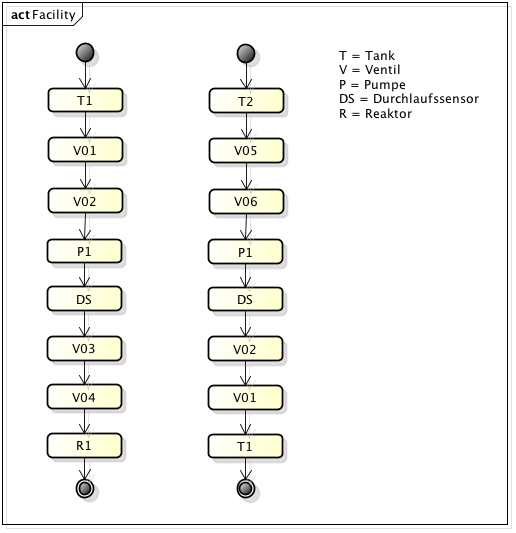
\includegraphics[width=0.7\textwidth]{graphics/konzept/UML_Activity.png}
		\caption{Abbildung der Wege mittels Aktivitätsdiagramm}
		\label{fig:konz_UML_Activity}
\end{figure}\\
In Abbildung~\ref{fig:konz_UML_Activity} ist das erste Element der „Prozedur 1“ ein Tank (T1), gefolgt von der Öffnung zweier Ventile (V1, V2) und der Inbetriebnahme der Pumpe (P1). Danach ist die Messung des Durchflusssensor (DS1) gefolgt von der Öffnung weiterer Ventile (V3, V4) mit dem Ziel im Reaktor (R1). 
Mithilfe einer solchen Folge kann der Ablauf einer Prozedur genau bestimmt werden, um bei der Codegenerierung diese erstellen zu können. 

\section{Zusammenfassung}
\todo{Zusammenfassung Kapitel 3}